\pah{18-01-2019}
\section{Some Definitions}\label{sec:bounds}
\underline{Upper bound}: $S \subset \mathbb{R}$, $a \in \mathbb{R}$\\
What does it mean for $a$ to be an upper bound of $S$?\\
As it was already done \hyperref[sec:ub]{here}, you may know what the exact definition is but nevertheless, it is good practise to have an intuition.\\
With reals, what often helps is the \textit{number line}, with which we are all familiar.\\
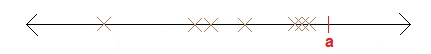
\includegraphics[width=18 cm]{images/upperbound.jpg}\\
\phantom{ } \hfill (Here, the $\times$s represent elements of $S$)\\
What the above diagram shows is that the number $a$ lies on the right of \textit{every} element of the set. It might now feel natural to write the definition that we saw before:
\begin{center}
    \highlight{$a$ is an upper bound of $S$ if: $\forall x \in S(x \le a)$}
\end{center}
Similarly, what can we say if $a$ is \textbf{\textit{not}} an upper bound of $S$? Once again, we may draw a number line as follows:\\
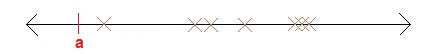
\includegraphics[width=18 cm]{images/lowerboundfalse.jpg}\\
In the above case, $a$ is certainly not the upper bound. However, is this the only way? The above diagram shows that $a$ is to the left of \textit{every} element of $S$. What if there's a situation like below:\\
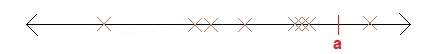
\includegraphics[width=18 cm]{images/lowerbound.jpg}\\
In this case as well, $a$ is \textit{\textbf{not}} an upper bound. Therefore, it not necessary that \textit{every} element of $S$ be greater than $a$, just \textit{one} would suffice. Now, we may write that:
\begin{center}
    \highlight{$a$ is not an upper bound of $S$ if: $\exists x \in S(a < x)$}
\end{center}
Of course, as we had already seen \hyperref[sec:negquant]{negating quantifiers} before, this was quite straightforward. The purpose of this activity had mainly been to illustrate the use of number lines and intuition.

\hrulefill
\exercise{Do the same for lower bounds.}

\hrulefill

\subsection{Proper way of writing a definition}\label{ssec:properdef}
\nopagebreak
\begin{enumerate}[label=(\arabic*)]
    \item Let $a\in \mathbb{R}, S\subset \mathbb{R}.$\\
    We say $a$ is a lower bound of $S$ \textbf{in $\mathbb{R}$} if:\\
    $\forall x \in S(a \le x).$
    %
    \item Let $S\subset \mathbb{R}$.\\
    We say that $S$ has a lower bound \textbf{in $\mathbb{R}$} if:\\
    $\exists a \in \mathbb{R}\big(\forall x \in S(a \le x)\big)$
\end{enumerate}

Just like how we'd negated a complicated statement, the procedure of writing a definition is quite similar.\\
Begin with the last line as you know what the property is supposed to be. 
\begin{center}
    \highlight{$\forall x \in S(a \le x).$}
\end{center}
The above statement involves three \textit{characters}: $x$, $S$ and $a$. It is clear what $x$ is as it's mentioned in the statement itself. The other two characters will have to be introduced. It is now immediately clear what we must write:
\begin{center}
    \highlight{%
    Let $a\in \mathbb{R}, S\subset \mathbb{R}.$\\
    $\forall x \in S(a \le x).$}
\end{center}
Now, all we are left with is just to tell the reader what is it that we are defining.
\begin{center}
    \highlight{%
    Let $a\in \mathbb{R}, S\subset \mathbb{R}.$\\
    We say $a$ is a lower bound of $S$ if:\\
    $\forall x \in S(a \le x).$}
\end{center}
Note that this line came second as the line uses the characters $a$ and $S$.\\
If you look at the two definitions above, you may notice that in the second definition, ``$a\in \mathbb{R}$" was not part of the introduction. This is correct because the third line tells us what $a$ is. (This is similar to how we never introduce $x$ before.)\\~\\
If you see the final statement of definition (2), the inner statement is just taken from the previous definition. This shows how one builds up definitions and that an intermediate step could have just been to write:
\begin{center}
    \highlight{$\exists a \in \mathbb{R}(a $ is a lower bound of $S)$}
\end{center}
Which is then followed by the definition of $a$ being a lower bound of $S$.
%
\section{Proofs versus Counterexamples}\label{sec:pvsce}
Consider the statement:
\begin{center}
    \simpleexample{Every non-empty subset of $\mathbb{R}$ has a lower bound in $\mathbb{R}$.\\
    That is: $\forall S \subset \mathbb{R}, S \neq \emptyset\Big(\exists a \in \mathbb{R}\big(\forall x \in S(a\le x)\big)\Big)$}
\end{center}
Is the above statement true? If yes, how would we show that? If no, then how would we show that?\\
The statement starts with the \hyperref[ssec:univquant]{"for all" quantifier}. Therefore, what it claims afterwards must hold for \textit{all} non-empty subsets $S$ for it to be true. This means that to show that it is false, all one would have to do is to find a single case where it does not hold, that is, a counterexample.\\
This reasoning is also consistent with the way we negated quantifiers before. Let us write the negation of the above statement.
\begin{center}
    \simpleexample{$\exists S \subset \mathbb{R}, S \neq \emptyset\Big(\forall a \in \mathbb{R}\big(\exists x \in S(x < a )\big)\Big)$\\
    That is: There is a non-empty subset of $\mathbb{R}$ that does \textit{not} have a lower bound in $\mathbb{R}$.}
\end{center}
Note an important thing: even in the negation, we're still saying \simpleexample{$S\neq\emptyset$}. This is because I made my original statement about non-empty subsets of $\mathbb{R}$; therefore, if you say that the inner-statement doesn't hold for the empty subset, you've not proven me wrong.\\
Another example of this would be:\\
\simpleexample{%
My claim: Chirag is the tallest student in this classroom.\\
To prove me wrong, you'd have to pick a \textit{\textbf{student}} in the room who is taller than Chirag. You would \textbf{\textit{not}} have proven me wrong if you pick some professor%
\footnote{ignoring the philosophical take that ``we're  all students in some way".}%
in the classroom and they happen to be taller than Chirag.
}\\
Now, going back to the original statement, let's try to prove it wrong. We have shown that all it would take to disprove the statement is to find a single counterexample. So, let us think of a non-empty subset that would not have a lower bound.\\~\\
In terms of the number line, what would this mean?\\
It would mean that no matter what real number $a$ that you choose, there would be an element of the set $S$ which is to the left of $a$. The picture would look something like:\\
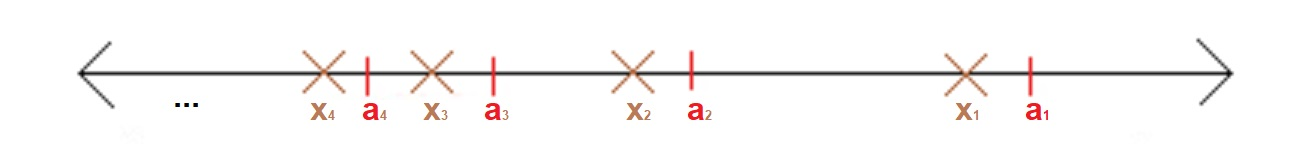
\includegraphics[width=18 cm]{images/nolowerbound.jpg}\\
Note that more than one element of $S$ can lie to the left of the $a$ you choose, the important thing is that \textit{at least} one does.\\
One simple counterexample can be $\mathbb{R}$ itself.

\hrulefill
\exercise{Given the above picture, come up with 5 counterexamples.}
\exercise{Prove that all the sets that you mentioned above do not have a lower bound in $\mathbb{R}$.}
\exercise{Is the statement true if we replace $\mathbb{R}$ with: (i) $\mathbb{N}$ (ii) $\mathbb{Z}$?}

\hrulefill

\highlight{\textbf{Claim: }
\begin{tabular}[t]{l}
     Let $S \subset \mathbb{R}, \cancel{S \neq \emptyset}$\\
     Suppose $S$ has a maximum.\\
     Then, $S$ is bounded above and $\operatorname{max}(S) = \operatorname{lub}(S)$.
\end{tabular}
}\\
In the above claim, I have struck out ``$S \neq \emptyset$", this is because that is redundant as $S$ having a maximum would imply that it's non-empty.\footnote{once again, recall that maximum demands the existence of a maximal element within the set itself.}\\
This is actually how one makes a theorem ``stronger". There are two ways of doing so:\\
(i) decrease the assumptions.\\
(ii) increase the conclusions.
%
\section{Well Ordering Principle}\label{sec:wop}
\highlight{\textbf{Axiom: }Every non-empty subset of $\mathbb{N}$ has a minimum.\\
That is: $\forall S \subset N, S \neq \emptyset\Big(\exists m \in S\big(\forall n \in S(m \le n)\big)\Big)$}\\
The above is known as well-ordering principle and is taken as an axiom.\\
It is easy to show that every subset of $\mathbb{N}$ would have a lower bound in $\mathbb{R}$. (1 would be a lower bound for every subset.) Well Ordering Principle is a stronger claim. If you feel it's obvious that a set having a lower bound should have a minimum, note that the same argument does not work for $\mathbb{Q}$.
%
\section{Intervals Notation}\label{sec:intervals}
Let $a, b \in \mathbb{R}$ for the following list:
\begin{enumerate}
    \item $(-\infty, \infty) = \mathbb{R}$
    \item $(-\infty, a) = \{x \in \mathbb{R}|x < a\}$
    \item $(-\infty, a] = \{x \in \mathbb{R}|x \le a\}$
    \item $(a, \infty) = \{x \in \mathbb{R}|a < x\}$
    \item $[a, \infty) = \{x \in \mathbb{R}|a \le x\}$
    \item $(a, b)$ 
    \begin{tabular}[t]{l}
        $=\{x \in \mathbb{R}|a < x$ and $x < b\}$  \\
        $=\{x \in \mathbb{R}|a < x\}$ and $\{x \in \mathbb{R}|x < b\}$ \\
        $=\{x \in \mathbb{R}|a < x\} \cap \{x \in \mathbb{R}|x < b\}$ \\
        $= (-\infty, b) \cap (a, \infty)$
    \end{tabular}
    \item $(a, b]= (-\infty, b] \cap (a, \infty)$
    \item $[a, b)= (-\infty, b) \cap [a, \infty)$
    \item $[a, b]= (-\infty, b] \cap [a, \infty)$
\end{enumerate}
Note that $\infty$ is just a symbol that has been used in some sort of notation, nothing more.